\subsection{Experimental design}

\subsubsection{Conceptual basis}

An ideal analysis of regex behavioral similarity would use subsumption or containment analysis. However, we struggled to find a tool that could facilitate such an analysis. Further, regular expressions in code libraries (e.g., for Python, Java) are not the same as regular languages in formal language theory. Some features of regular expression libraries, such as backreferences, make the libraries more expressive than regular languages. This allows a regular expression pattern to match, for example, repeat words, such as ``cabcab", using the pattern {\tt ([a-z]+)\verb!\!1}. However, building an automaton to recognize such a pattern and to facilitate containment analysis, is infeasible.
For these reasons, we developed a similarity analysis based on string matching.

\begin{figure}[tb]
\centering
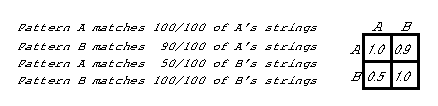
\includegraphics[height=0.6in]{nontex/illustrations/minimalMatrix.eps}
\caption{A similarity matrix created by counting strings matched}
\label{fig:minimalMatrix}
\end{figure}

\begin{figure}[tb]
\centering
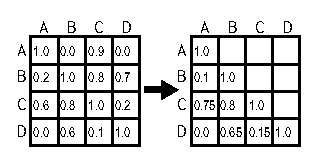
\includegraphics[width=0.7\columnwidth]{nontex/illustrations/matrixToGraph.eps}
\vspace{-6pt}
\caption{Creating a similarity graph from a similarity matrix}
\vspace{-6pt}
\label{fig:matrixToGraph}
\end{figure}



\subsubsection{Overview of process}

Our similarity analysis clusters regular expressions by their behavioral similarity on matched strings.
Consider two unspecified patterns {\tt A} and {\tt B}, a set {\tt mA} of 100 strings that pattern {\tt A} matches, and a set {\tt mB} of 100 strings that pattern {\tt B} matches.
If pattern {\tt B} matches 90 of the 100 strings in the set {\tt mA}, then {\tt B} is 90\% similar to {\tt A}.
If pattern {\tt A} only matches 50 of the strings in {\tt mB}, then {\tt A} is 50\% similar to {\tt B}.
We use similarity scores to create a similarity matrix as shown in Figure~\ref{fig:minimalMatrix}.
In row {\tt A}, column {\tt B} we see that {\tt B} is 90\% similar to {\tt A}.
In row {\tt B}, column {\tt A}, we see that {\tt A} is 50\% similar to {\tt B}.  Each pattern is always 100\% similar to itself, by definition.

Once the similarity matrix is built, the values of cells reflected across the diagonal of the matrix are averaged to create a half-matrix of undirected similarity edges, as illustrated in Figure~\ref{fig:matrixToGraph}.
This facilitates clustering using the  Markov Clustering (MCL) algorithm\footurl{http://micans.org/mcl/}.
We chose MCL  because it offers a fast and tunable way to cluster items by similarity and it is particularly useful when the number of clusters is not known \emph{a priori}.


In the implementation, strings are generated for each pattern using Rex~\cite{rex}.  Rex generates matching strings by representing the regular expression as an automaton, and then passing that automation to a constraint solver that generates members for it\footurl{http://research.microsoft.com/en-us/projects/rex/}.  If the regex matches a finite set of strings smaller than 400, Rex will produce a list of all possible strings.
Our goal is to generate 400 strings for each pattern to balance the runtime of the similarity analysis with the precision of the similarity calculations.

For clustering, we prune the similarity matrix to retain all similarity values greater than or equal to 0.75, setting the rest to zero, and then using MCL.
This threshold was selected based on recommendations in the MCL manual. The impact of lowering the threshold would likely result  in either the same number of more diverse clusters, or a larger number of clusters, but is unlikely to markedly change the largest clusters or their summaries, which are the focus of our analysis for \todoMid{some research question reference}.
, but further study is needed to substantiate this claim.
We also note that MCL can also be tuned using many parameters, including inflation and filtering out all but the top-k edges for each node.
After exploring the quality of the clusters using various tuning parameter combinations, the best clusters (by inspection) were found using an inflation value of 1.8 and k=83.   The top 100 clusters are categorized by inspection into six categories of behavior.

The end result is clusters and categories of highly behaviorally similar regular expressions, though we note that this approach has a tendency to over-approximate the similarity of two regexes. We measure similarity based on a finite set of generated strings, but some regexes  match an infinite set (e.g., \verb!ab*c!), so measuring similarity based on the first 400 strings may lead to an artificially high similarity value. To mitigate this threat, we chose a large number of generated strings for each regex, but future work includes exploring other approaches to computing regex similarity.


